\section{Software Design} \label{ch:SWdesign}

Gennem designprocessen har fokus for softwaredesignet været at parallelisere de vigtigste opgaver i tråde, samt holde ressourceforbruget nede, da memory på DevKit8000 er begrænset. Softwaredesignet er lavet på baggrund af sekvensdiagrammer for relavante use cases på side \pageref{P-sec:usecasebeskrivelser} i projektdokumentationen, så omfanget af softwarearbejdet var nogenlunde kendt på forhånd.

\subsection{Sekvensdiagrammer}

\begin{figure}[h!]
\centering
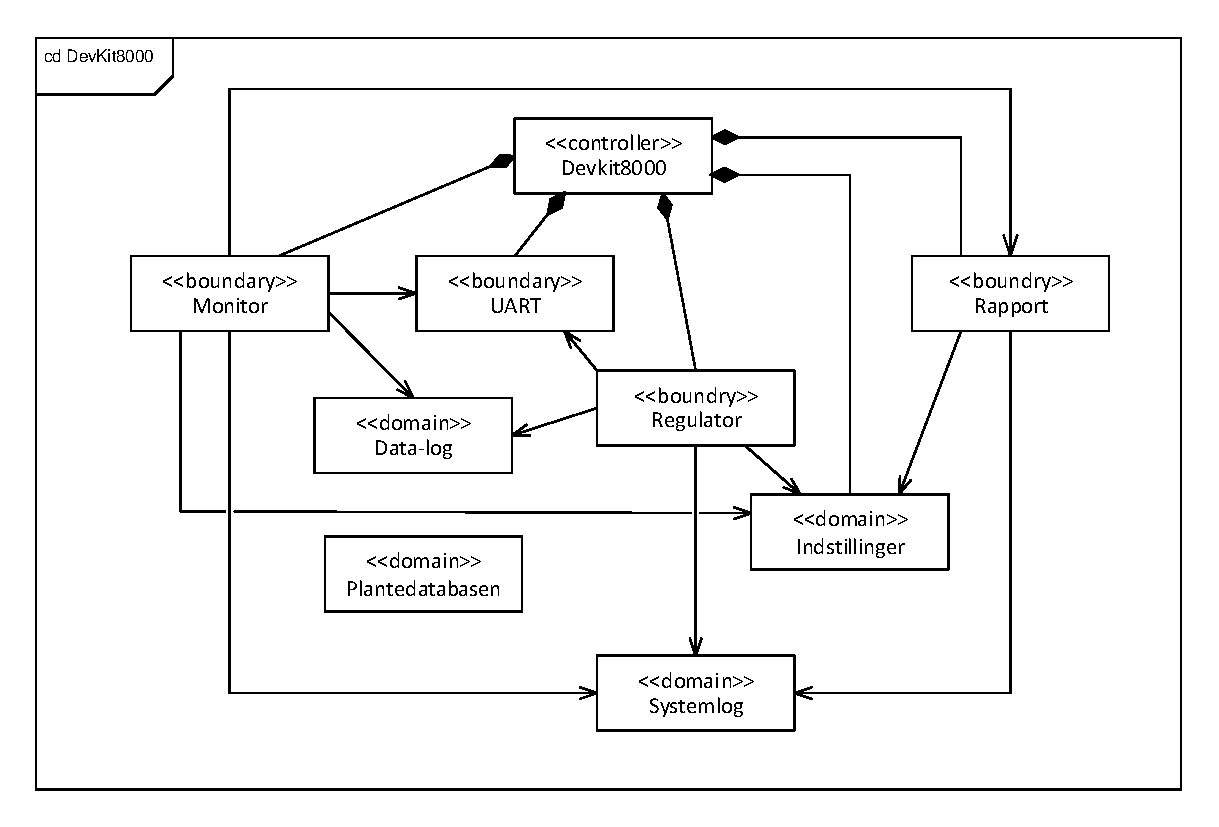
\includegraphics[width=\textwidth - 1 cm]{../fig/UML_autogreen.pdf}
\caption{Klassediagram for DevKit8000}
\label{fig:applikationsmodel} 
\end{figure}

På Figur \ref{fig:applikationsmodel} ses klassediagram fra systemarkitekturen, som ligger til grundlag for konstruktionen af sekvensdiagrammer. Sekvensdiagrammernes funktion er, at klarlægge de enkelte klassers metoder og associationer, samt at give et overblik over klassernes funktionalitet.

\clearpage

\subsection{Klassebeskrivelser}

\begin{figure}[ht]
\centering
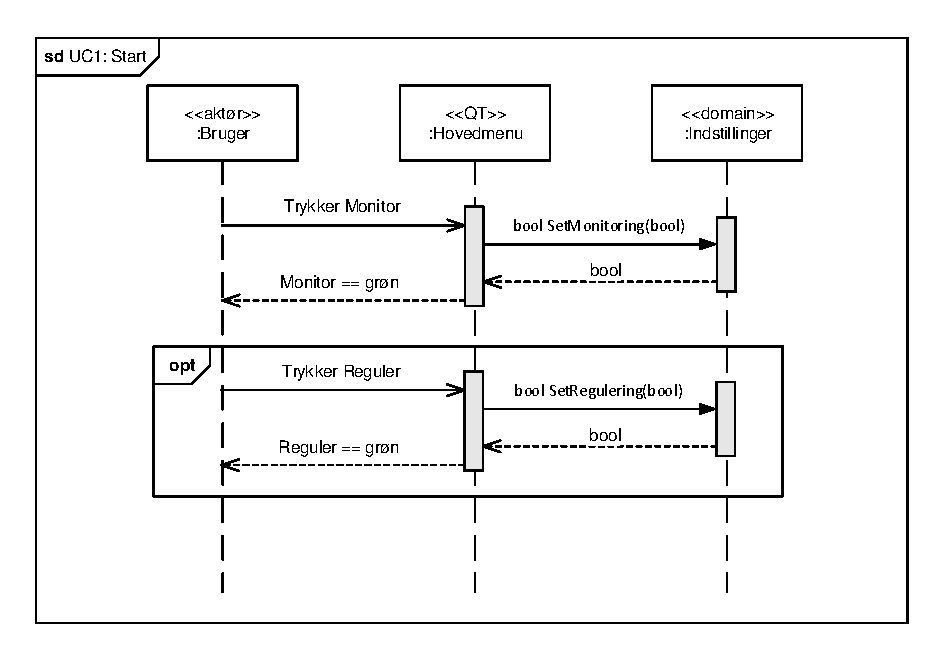
\includegraphics[width=\textwidth - 1 cm]{../fig/SD_autoGreen_UC_1_Start.pdf}
\caption{Eksempel for sekvensdiagram.}
\label{fig:sekvens} 
\end{figure}

Under arbejdet med sekvensdiagrammerne (se Figur \ref{fig:sekvens}), var det nødvendigt med mindre tests af funktionaliteten og virkemåden i QT \cite{lib:QT_doc}. Ud fra disse tests, blev QT set som et bindeled mellem grundsystemets klasser, som fx monitor og regulator.
Dette lagde grund for klassebeskrivelser, men ikke beskrivelser for QT-klasserne, da gruppen valgte at udskyde dette til implementationsfasen. Det store fokus har været på trådhåndtering i monitor og regulatoren, samt valg af datastrukturer. 
Det endelige design omfatter grundsystemets opbygning og de interne forbindelser mellem klasserne.

\subsection{Datastruktur}

Valget af datastruktur (se \nameref{P-sec:DoublyLinkedList} på side \pageref{P-sec:DoublyLinkedList} i dokumentationen) til lagring af data forskellige steder i systemet, er valgt af hensyn til simplicitet. 
Det blev bestemt at bruge doublylinkedlist, da den primære brug af datastrukturen skulle være at tilgå det senest tilføjede element. 
Dette gør doublylinkedlist til et optimalt valg, da man kan tilgå både første og sidste element, igennem head- og tailpointere. For ikke at overkomplicere systemet med forskellige datastrukturer, blev det vedtaget, at doublylinkedlist skulle bruges som datastruktur i alle andre lagringsområder i systemet, foruden indstillinger. 

Indstillinger blev implementeret som en klasse, da den havde flere forskellige slags information der skulle lagres. Dataloggen skulle indeholde de samme data i alle noder (se Figur \ref{fig:DoublyLinkedList}), mens indstillinger kun skulle indeholde én af hver information, fx om varmelegeme skal anvendes eller ej.

\clearpage

\begin{figure}[ht]
\centering
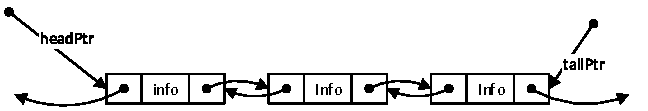
\includegraphics[width=\textwidth - 1 cm]{../fig/linkedNodes.pdf}
\caption{Eksempel på en DoublyLinkedList}
\label{fig:DoublyLinkedList}
\end{figure}

Der blev besluttet at køre flere tråde på systemet for at give mulighed for softwaren at arbejde parallelt. 
Da det blev bestemt at køre regulator og monitor i hver deres tråd, var det vigtigt at sikre de tilgående klasser som fx UART. 
Idet både monitor og regulator bruger UART'en til at hente og indsamle data fra, er det vigtigt at disse ikke kommer i konflikt over hvem der skal bruge den. Problemet blev løst ved brug af "mutual exclusion" også kendt som "mutexes", så kun en tråd kan tilgå klassens funktionalitet ad gangen. 
Til at oprette og køre tråde, blev pthread biblioteket anvendt, eftersom der allerede var kendskab til brugen af pthread fra undervisningen. 
Det var desuden sikkert, at pthreads fungerede på DevKit8000, da tråde er blevet testet på platformen gennem hele semesteret.

\subsection{Datatransmission}

Til transmission af data imellem DevKit8000 og PSoC Master, blev det besluttet at anvende UART. 
Denne beslutning blev taget pga. tidligere erfaringer med UART og dermed ville det være oplagt at bruge denne kommunikationsform. 
DevKit8000 har 3 RS-232 porte, og der er mulighed for at mappe UART'en til andre ben på addon-boardet (se \nameref{P-sec:uart_impl_opsatning} på side \pageref{P-sec:uart_impl_opsatning} i projektdokumentation).

I systemet var der brug for at kende tidsstemplingen på det indsamlede data, som hentes fra drivhuset. Der kunne være brugt en tråd, som hele tiden tæller tiden op i system, men sandsynligheden for præcisionsproblemer ville være stor. 
På DevKit8000 kører der en Linux-distribution der allerede har en timer, som holder fint styr på tiden. Derfor blev det besluttet at bruge denne timer, for gøre systemet mere simpelt.

\subsection{Intertrådskommunikation}

For at få en bedre ide om hvad systemet laver og hvilke systemhændelser som finder sted, blev der lavet en systemlog. 
I forbindelse med dette, skulle der oprettes en ekstra tråd, som modtager beskeder fra de klasser, der har relevante tilbagemelding om hændelser i systemet. Et eksempel er, fx når regulator vurderer at der er for varmt i drivhuset. For at realisere dette, blev der oprettet en messagequeue, som beskeder kan sendes til. Beskederne bliver taget ud og gemt i DoublyLinkedList'en.

Der skulle også være mulighed for at få tilsendt e-mails fra systemet. Der defineres to typer e-mails: En advarsels e-mail, som bliver sendt, hvis klimaet i drivhuset når et kritisk niveau, og en daglig e-mail, som beskriver hvad der er forgået inden for de sidste 24 timer. Brugeren kan selv styre hvilke e-mails der ønskes. Der er plads til at e-mails kan sendes til maksimalt tre e-mailadresser, som der indstilles i e-mailmenuen (Se beskrivelse i \nameref{P-sec:mailmenu} på side \pageref{P-sec:mailmenu} i dokumentation.)

I AutoGreen er der en plantedatabase, som skal indeholde prædefinerede planter, som kan indsættes i det virtuelle drivhus. Denne database skal også bruge DoublyLinkedList'en til at gemme de prædefinerede planter. Ideen bag plantedatabasen er, at kunne samle en række prædefinerede planter og en række selvdefinerede planter, som brugeren har mulighed for at tilføje til det virtuelle drivhus. 

\clearpage